\documentclass[a4paper, 12pt]{article}

\usepackage[T1]{fontenc}
\usepackage{paralist}
\usepackage{amsmath}
\usepackage{romannum}
\usepackage{graphicx}
\newtheorem{definition}{Definition}[section]
\graphicspath{{./images/}}
\newcommand{\head}[1]{\textnormal{\textbf{#1}}}

\begin{document}

\title{ACCT-111 Principles of Accounting} \author{Luka Trikha}
\maketitle
\begin{figure}[h]
    \centering
    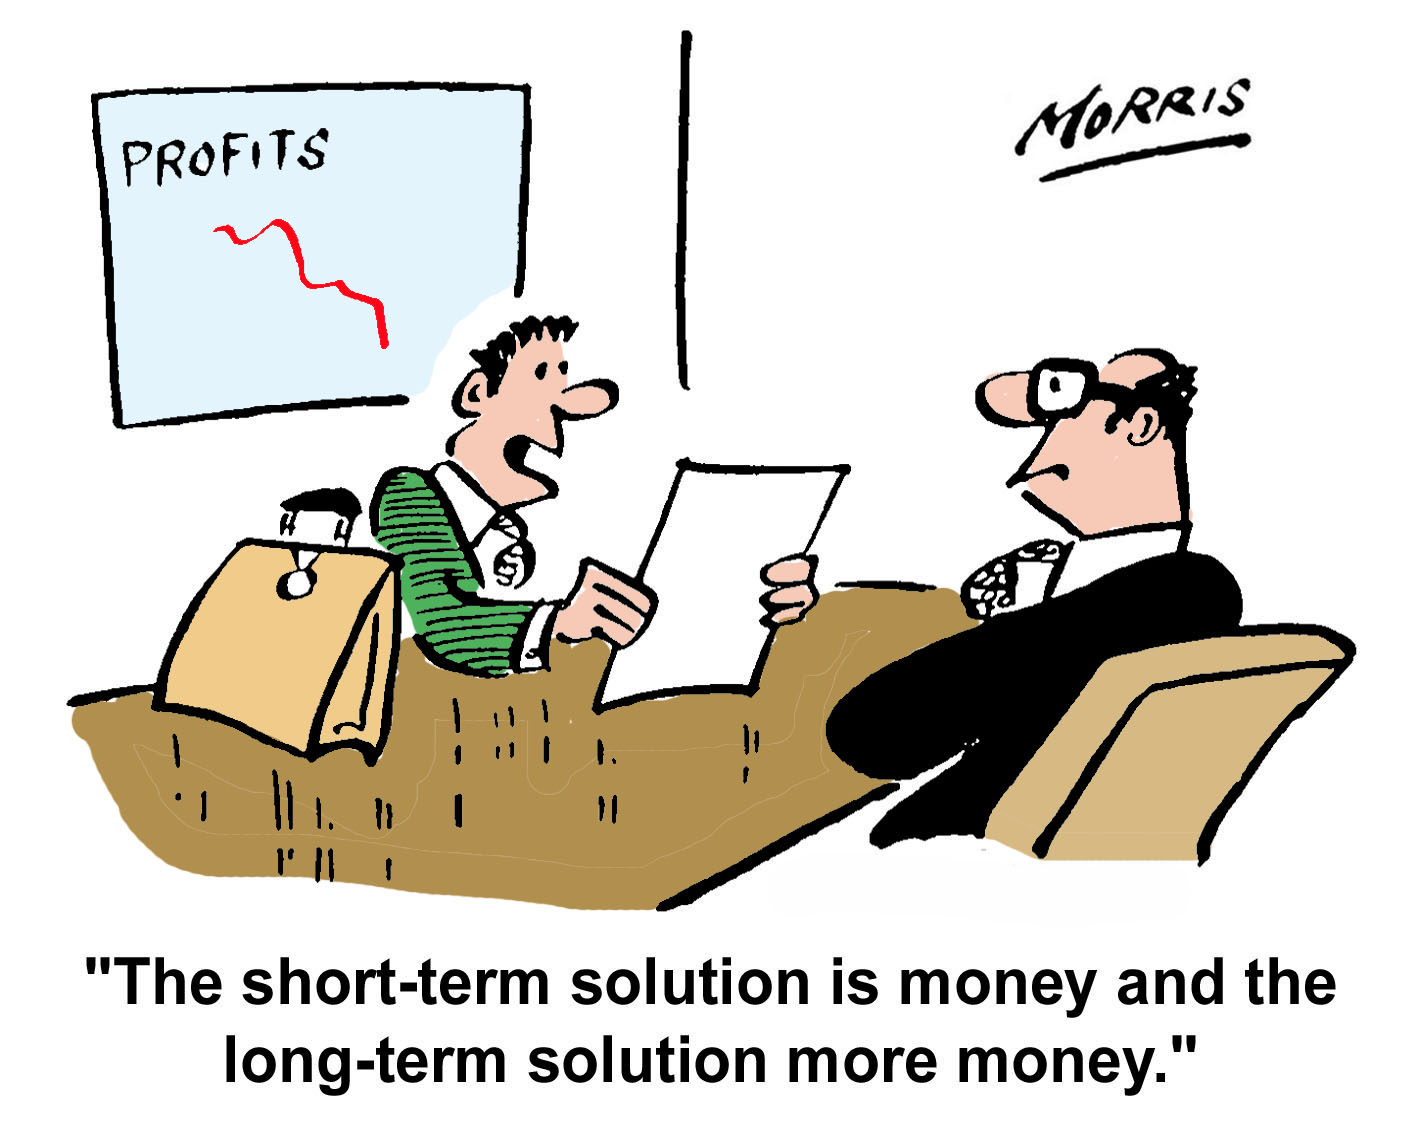
\includegraphics{cartoon.jpg}
\end{figure}
\newpage

\tableofcontents
\newpage

\section{Accounting and the Business Environment}
\subsection{Why is Accounting Important?}
\textbf{Accounting} is the information system that measures business activities,
processes the information into reports, and communicates the results to decision
makers.

Accounting can be divided into two major fields, \textit{financial accounting}
and \textit{managerial accounting}.\\[2mm]
\textbf{Financial accounting} provides information for external decision makers
such as outside investors, lenders, customers, and the federal government.\\[2mm]
\textbf{Managerial accounting} focuses on information for internal decision
makers, such as the company's managers and employees.
Other definitions to note:
\begin{compactitem}
    \item \textbf{Creditor} are a person or business to whom a business owes
        money.
    \item \textbf{Certified public accountant (CPA)} are professional accountants
        who serve the general public.
    \item \textbf{Certified management accountants (CMA)} are professionals who
        work for a single company.
\end{compactitem}

\subsection{What are the Organizations and Rules that Govern Accounting?}
There are different private and federal organizations which dictate accounting
standards in the united states.

The \textbf{Financial Accounting Standards Board (FASB)} is a privately funded
organization that oversees the creation and governance of accounting standards
in the United States.

The \textbf{Securities and Exchange Commission(SEC)} is a U.S. Government agency
that oversees the U.S. Financial markets, as well as oversees organizations that
set standards (like FASB).

The guidelines for accounting information are called the \textbf{Generally Accepted
Accounting Principles (GAAP}. It was created and governed by the FASB. GAAP rests
on a conceptual framework that identifies the objectives, characteristics,
elements, and implementation of financial statements and creates the acceptable
accounting practices. The goal of the GAAP is to provide \textbf{faithful
representation} of data. Faithful representation is information that is complete,
neutral and free from material error.

Time to look at different types of economic entities. Below is a chart that
goes into depth the various different business organizations that can be found.

\begin{figure}[h]
    \centering
    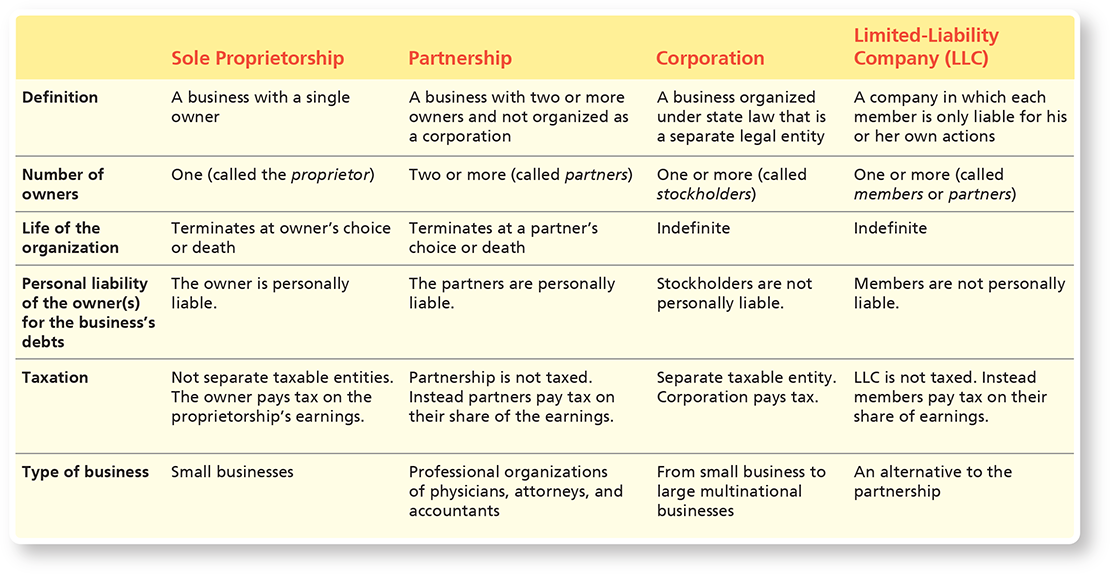
\includegraphics[width=13.0cm, height=7cm]{business_organizations.png}
    \caption{Table of four different business organizations and the characteristics
    of each organization}
    \label{fig:bus_org1}
\end{figure}

When starting to note the costs you are spending/receiving, it is important to
use the \textbf{cost principle}. The cost principle states that any acquired
assets and services should be recorded at their actual host (or \emph{
historical cost}, aka the price \emph{actually} paid or transaction on a receipt.
We do this because it is a reliable measurement when looking back at transactions.

Noting historical costs is also good for \textbf{going concern assumption}, which
is the assumption that a business will remain in operation long enough to use
existing resources for their intended purposes.

The costs we keep track of are in dollar units, since that is the medium of 
exchange in the U.S. Even though inflation can decrease the value of the dollar,
accountants assume the dollar's purchasing power is stable, and that is the essence
of \textbf{monetary unit assumption}. Monetary unit assumption requires items
on a financial statement be in units of monetary value.

So far, these principals are the ones that follow U.S. GAAP and are traded on
the U.S stock exchange. But if a company deals with international partners, then
they will publish financial statements using the \textbf{International Financial
Reporting Standards (IFRS)}, which are published by the \textbf{International
Accounting Standards Board (IASB)}. IFRS is a set of global accounting standards
that are used by more than 166 nations/jurisdictions and are usually less specific
compared to U.S. GAAP. Another difference is that IFRS allows periodic revaluation
of certain assets and liabilities to restate financial statements to market value
rather than keeping the financial statements at historical cost.

There can be different ethical concerns when dealing with business and what they
wish to disclose to the public/investors. This is why the SEC requires publicly
help companies to have their financial statements audited by independent
accountants. An audit is an examination of a company's financial statements and
records. It is then up to the independent accountant to issue an opinion that 
states whether or not the financial statements give a fair picture of the 
company's financial situation.

There have been two major outcomes form scandalous accounting actions. The
\textbf{Sarbanes-Oxley Act (SOX)} requires management to review internal control
and take responsibility for the accuracy and completeness of their financial
reports. The SOX also created the \textbf{Public Company Accounting Oversight Board
(PCAOB)} to monitor the work of independent accountants who audit public companies.

\subsection{What is the Accounting Equation?}
The \textbf{accounting equation} measures the resources of the business
(what the business owns or has control of) and the claims to those resources (
what the business owes to creditors and to the owners). The equation is $Assets = 
Liabilities + Equity$. Since this is an \emph{equation}, both sides need to be
equal to each other, that is, the total amount in $assets$ must equal the total
amount of $liabilities + equity$. This is also called "balancing the books."

An \textbf{asset} are economical resources that are expected to benefit the
business in the future and something the business owns or has control of. A few
examples of what an asset is are:
\begin{itemize}
    \item cash
    \item merchandise inventory
    \item furniture
    \item land
    \item equipment
\end{itemize}

A \textbf{liability} are debts that are owed to creditors. They are something
the business owes and represent the creditors' claim on the business's assets.
Most of the times, liabilities have the word \emph{payable} in their titles.
Examples of liabilities are:
\begin{itemize}
    \item accounts payable
    \item notes payable
    \item salaries payable
    \item a creditor who has loaned money to a business has a claim to some of
        the business's assets until the business pays the debt.
\end{itemize}

\textbf{Equity} is the owner's claim to the assets of the business. This is also
called \emph{owner's equity}. Equity represents the amount of assets that are
left over after the company has paid its liabilities. It is the company's net


When an owner of a business contributes to a business (cash, equipment, etc.), 
this is called \textbf{owner's capital}. This can also be called common stock.
When a business makes earnings from delivering goods or services to customers,
this is called \textbf{revenue}. Some examples of revenue are:
\begin{itemize}
    \item sales revenue
    \item service revenue
    \item rent revenue
\end{itemize}
Again, these are ways that equity increases for the business.

Equity can also decrease when an owner makes a withdrawal or the business has
expenses it needs to pay.

\textbf{Owner's \emph{withdrawals}} or \textbf{\emph{drawings}} are payments of
equity (usually in cash) to the owner. Owner withdrawals are the opposite of
owner contribution. Owner withdrawals are \emph{not} expenses. Owner's drawings
can also be known as dividends.

\textbf{Expenses} are the costs of selling goods or services. Some examples of
expenses are:
\begin{itemize}
    \item rent expense
    \item salaries expense
    \item advertising expense
    \item utilities expense
\end{itemize}

While looking at this as a whole, we can calculate a \textbf{net income} or a 
\textbf{net loss}. A net income is when the difference between revenue and 
expenses is positive ($revenue - expenses = +$), while net loss is when the
difference between revenue and expenses are negative ($revenue - expenses = -$).

As a reminder, assets are what a company has, liabilities are what a 
company owes, and equity is the net worth of the company.

\subsection{How do you Analyze a Transaction?}
A transaction is any event that affects the financial position of the business
\emph{and} can be measured with faithful representation (trustworthy exchange
between goods and services, expenses, etc.) Accountants do not note any type of
financial anomaly that appear (financial booms, recession, inflation, etc.),
accountants only note down what is of monetary value and can be measured reliably.
Furthermore, they will only account for the true cost of the transaction, ignoring
\emph{potential} value and only focusing on what goods and services are worth at
the time the transaction occurred.

When looking at transactions with a business, you must always look in the eyes
of the business, not the owner or customer.

There can be two different types of assets/liabilities you can see when looking
at a transaction, \textbf{accounts payable} and \textbf{accounts receivable}.

Accounts payable is a short-term \emph{liability} that will be paid in the future.
This is when a business obtains an asset but does not pay right away, instead,
the business promises to pay in the future (like credit).

Accounts receivable (\emph{equity}) is when a company give away goods or services, and is promised
revenue (cash) from the customer in the future.

\subsection{How do you Prepare Financial Statements?}
In order to determine whether a business is profitable or not, an analysis of 
\textbf{financial statements} are required. There are four different financial 
statements that need to be prepared in order to make decisions. All four documents
are prepared in an ordered list as seen in figure \ref{fig:fin_state1}.
\begin{figure}
    \centering
    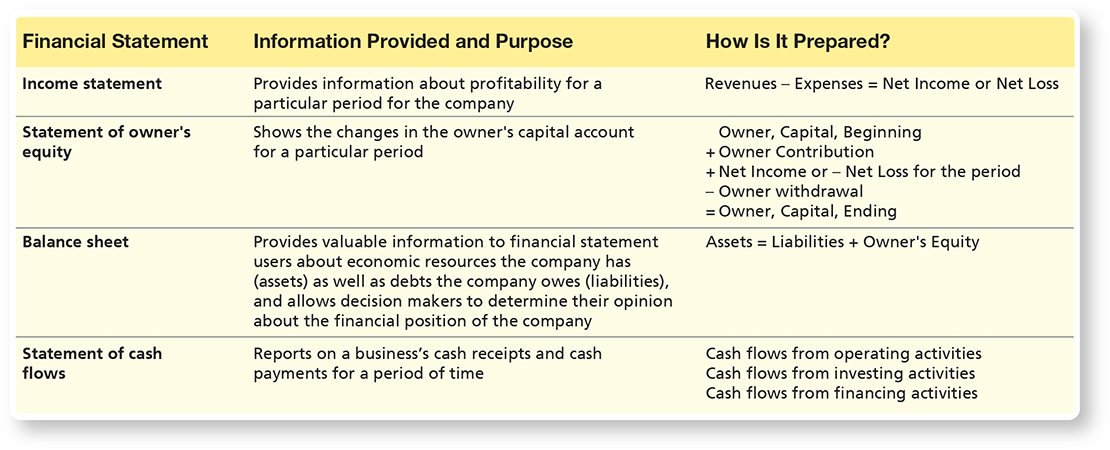
\includegraphics[width=13.0cm, height=7.0cm]{financial_statements.png}
    \caption{Ordered list of how financial statement documents should be prepared}
    \label{fig:fin_state1}
\end{figure}

\subsubsection{Income statements}
An income statement (also called \emph{statement of earnings} is a summary of a
business entity's revenues and expenses for a period of time (months, quarters,
yearly). Income statement tells us whether the business:
\begin{itemize}
    \item has a \emph{net income} (total revenue is greater than total expenses)
    \item has a \emph{net loss} (total expenses are greater than total revenue)
\end{itemize}
\textbf{\emph{Only}} revenues and expenses are reported on an income statement.
Information on what an income statement should have is shown in figure
\ref{fig:income_state1}
\begin{figure}
    \centering
    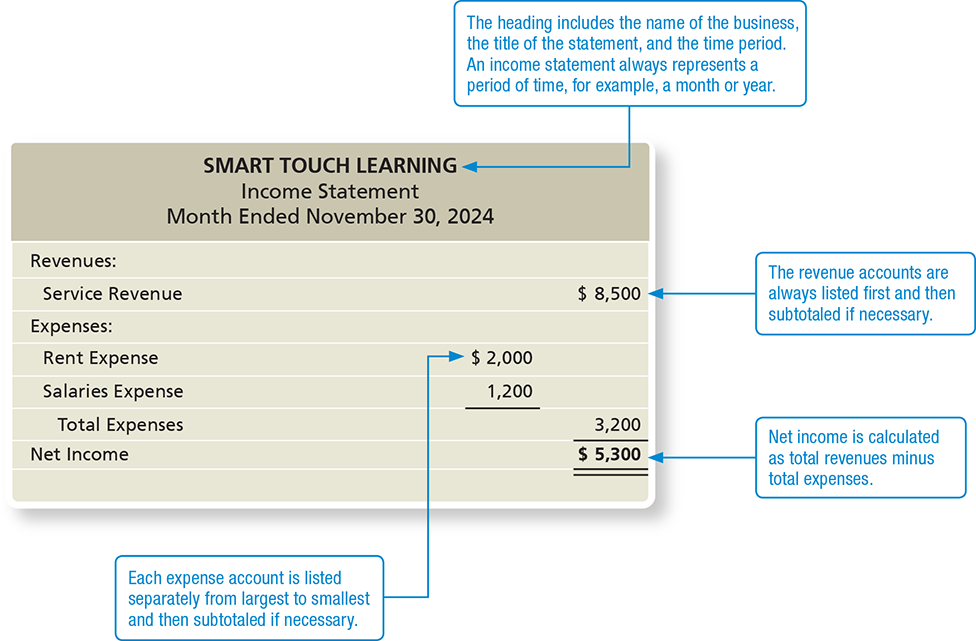
\includegraphics[height=10.0cm, width=13.0cm]{income_statement.png}
    \caption{Similar information every income statement should have}
    \label{fig:income_state1}
\end{figure}

\subsubsection{Statement of Owner's Equity}
A statement of owner's equity shows the changes in owner's capital for a
business entity for a period of time (months, quarters, yearly). This document
is built upon the income statement. See figure \ref{fig:owner_equity} a
reference.
\begin{figure}[h]
    \centering
    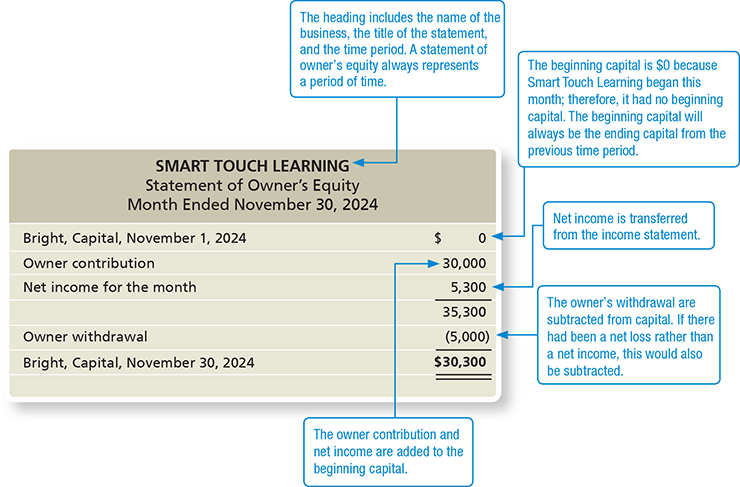
\includegraphics[height=10.0cm, width=13.0cm]{owners_equity.png}
    \caption{Similar information every owner's equity should have}
    \label{fig:owner_equity}
\end{figure}

\subsubsection{Balance Sheet}
Also known as the \emph{statement of financial position}, the balance sheet lists
a business entity's assets, liabilities, and owner's equity for a period of time
(months, quarters, yearly). Balance sheets are seen as a snapshot of the business
entity, and is used by investors or creditors to quickly assess the overall 
health of a business. Figure \ref{fig:balance_sheet} shows an example of a balance statement.
\begin{figure}[t]
    \centering
    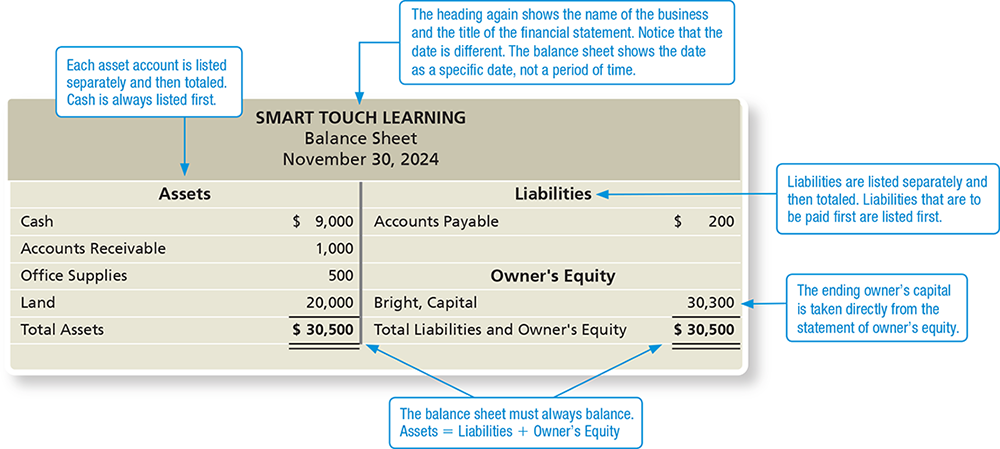
\includegraphics[height=8.0cm, width=13.0cm]{balance_statement.png}
    \caption{Similar information every balance sheet should have}
    \label{fig:balance_sheet}
\end{figure}

\subsubsection{Statement of Cash Flow}
Statements of cash flow reports cash coming in (positive) and going out (negative).
If a transaction does not involve cash (buying supplies on account), then it
will not be reported in this statement. This statement is to analyze net
increases or decreases during a period of time (months, quarters, yearly).
Cash flow statements are divided into three sections:
\begin{itemize}
    \item \textbf{Operating activities} involve cash payments for expenses.
    \item \textbf{Investing activities} involve the cash purchase and sale of
        land and equipment.
    \item \textbf{Financial activities} involve cash contributions by the owner,
        cash withdrawals paid to the owner, cash received from borrowing, and
        cash paid when loans are repaid.
\end{itemize}
Figure \ref{fig:cash_flow} how a cash flow statement looks like.
\begin{figure}
    \centering
    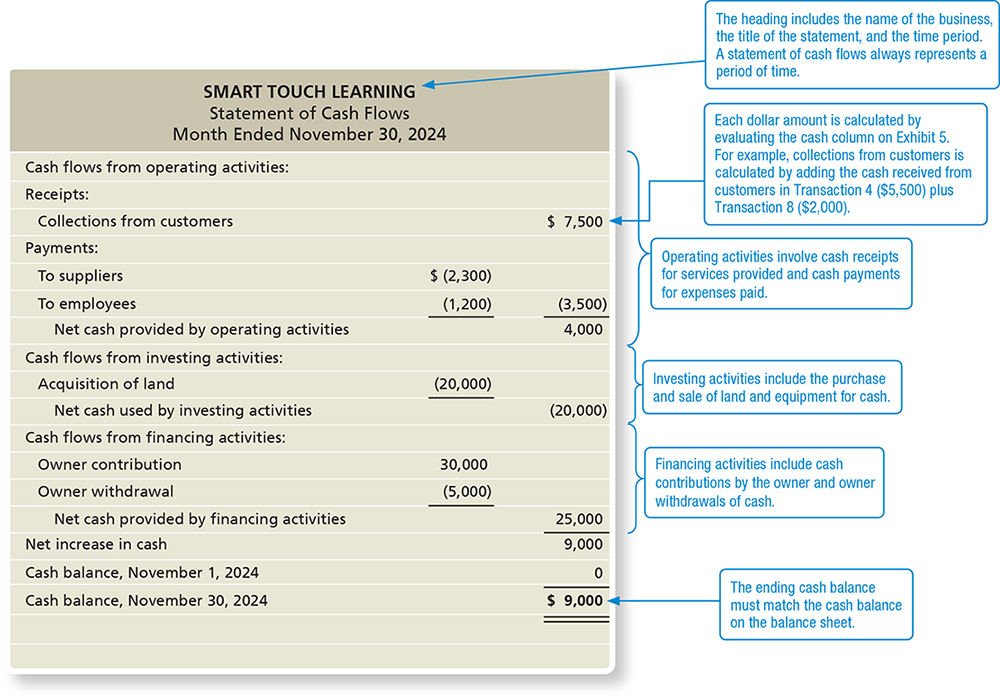
\includegraphics[height=10cm, width=13cm]{cash_flow.png}
    \caption{Similar information every cash flow should have}
    \label{fig:cash_flow}
\end{figure}

\subsection{How do you use Financial Statements to Evaluate Business Performance?}
When you have a financial statement, you can compute the \textbf{return on assets
(ROA)} to determine how well a company is performing. ROA measures how
profitably a company uses its assets. It is calculated by $Return on assets = 
\frac{\text{net income}} {\text{average total assets}}$. Average total assets is
calculated by adding the beginning and ending total assets for the time period
and diving by two.
$\text{Average total assets} = \frac{\text{(beginning total assets + ending total
assets)}}{2}$.

\section{Recording Business Transactions}




\section{The Adjusting Process}
\end{document}
